\documentclass[a4paper]{article}

\usepackage[margin=1.2cm]{geometry}
\usepackage{xcolor}
\usepackage{tikz}
\usepackage{fontspec}

\setmainfont{DejaVu Sans}
\pagestyle{empty}

\definecolor{bgVeryLight}{HTML}{F6F5F8}
\definecolor{grayLight}{HTML}{9D9DA3}
\definecolor{grayMedium}{HTML}{5C5D64}
\definecolor{grayDark}{HTML}{232327}

\definecolor{navyDark}{HTML}{223450}
\definecolor{blueSlate}{HTML}{5F769B}
\definecolor{blueDeep}{HTML}{345D95}
\definecolor{blueSteel}{HTML}{5C86B9}
\definecolor{blueMedium}{HTML}{6390C2}
\definecolor{blueLight}{HTML}{B4D2EA}

\definecolor{greenMain}{HTML}{70AE61}
\definecolor{greenLight}{HTML}{ACCDA1}

\definecolor{yellowPale}{HTML}{F9DC8C}
\definecolor{yellowWarm}{HTML}{F7D375}
\definecolor{amberMain}{HTML}{DEA52C}

\definecolor{orangeMain}{HTML}{E8995A}
\definecolor{orangeDark}{HTML}{D8902C}
\definecolor{redOrange}{HTML}{D86A50}
\definecolor{brownOrange}{HTML}{9B592E}

\definecolor{lavenderLight}{HTML}{C7BCDA}
\definecolor{lavenderMuted}{HTML}{AAAFC9}

\begin{document}
    \begin{center}
        {\fontsize{22}{26}\selectfont Full Donut Palette from the Transformer Figure}
    \end{center}
    
    \vspace{0.3cm}
    
    \begin{center}
        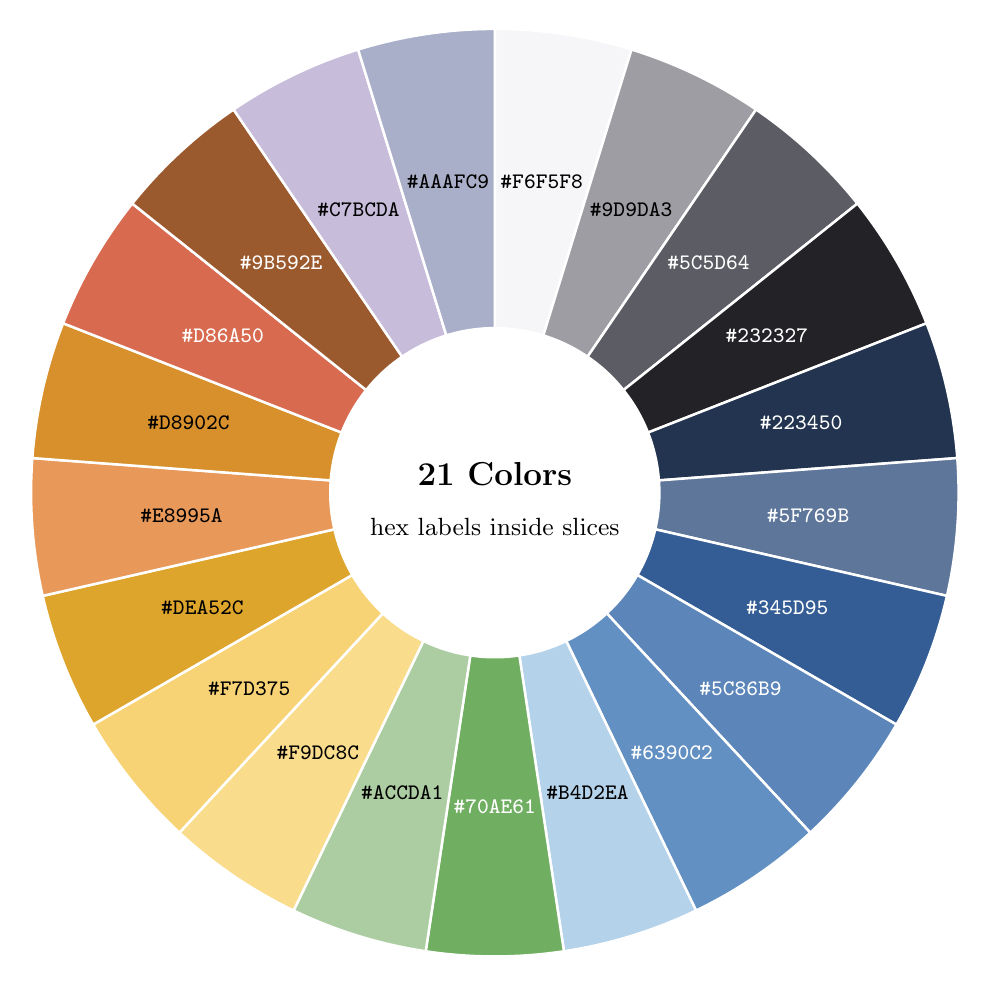
\begin{tikzpicture}[scale=0.95]

            \def\OuterRadius{6.2}
            \def\InnerRadius{2.2}
            \def\LabelRadius{4.2}
            
            \newcommand{\DonutSlice}[5]{%
                \fill[#1]
                (#2:\InnerRadius)
                arc[start angle=#2,end angle=#3,radius=\InnerRadius]
                --
                (#3:\OuterRadius)
                arc[start angle=#3,end angle=#2,radius=\OuterRadius]
                -- cycle;
                \draw[white, line width=0.9pt]
                (#2:\InnerRadius)
                arc[start angle=#2,end angle=#3,radius=\InnerRadius]
                --
                (#3:\OuterRadius)
                arc[start angle=#3,end angle=#2,radius=\OuterRadius]
                -- cycle;
                \node[
                    font=\ttfamily\footnotesize,
                    text=#4,
                    align=center
                ] at ({(#2+#3)/2}:\LabelRadius) {#5};
            }
            
            \DonutSlice{bgVeryLight}{90.000}{72.857}{black}{\#F6F5F8}
            \DonutSlice{grayLight}{72.857}{55.714}{black}{\#9D9DA3}
            \DonutSlice{grayMedium}{55.714}{38.571}{white}{\#5C5D64}
            \DonutSlice{grayDark}{38.571}{21.428}{white}{\#232327}
            
            \DonutSlice{navyDark}{21.428}{4.285}{white}{\#223450}
            \DonutSlice{blueSlate}{4.285}{-12.857}{white}{\#5F769B}
            \DonutSlice{blueDeep}{-12.857}{-30.000}{white}{\#345D95}
            \DonutSlice{blueSteel}{-30.000}{-47.142}{white}{\#5C86B9}
            \DonutSlice{blueMedium}{-47.142}{-64.285}{white}{\#6390C2}
            \DonutSlice{blueLight}{-64.285}{-81.428}{black}{\#B4D2EA}
            
            \DonutSlice{greenMain}{-81.428}{-98.571}{white}{\#70AE61}
            \DonutSlice{greenLight}{-98.571}{-115.714}{black}{\#ACCDA1}
            
            \DonutSlice{yellowPale}{-115.714}{-132.857}{black}{\#F9DC8C}
            \DonutSlice{yellowWarm}{-132.857}{-150.000}{black}{\#F7D375}
            \DonutSlice{amberMain}{-150.000}{-167.142}{black}{\#DEA52C}
            
            \DonutSlice{orangeMain}{-167.142}{-184.285}{black}{\#E8995A}
            \DonutSlice{orangeDark}{-184.285}{-201.428}{black}{\#D8902C}
            \DonutSlice{redOrange}{-201.428}{-218.571}{white}{\#D86A50}
            \DonutSlice{brownOrange}{-218.571}{-235.714}{white}{\#9B592E}
            
            \DonutSlice{lavenderLight}{-235.714}{-252.857}{black}{\#C7BCDA}
            \DonutSlice{lavenderMuted}{-252.857}{-270.000}{black}{\#AAAFC9}
            
            \fill[white] (0,0) circle (\InnerRadius);
            
            \node[align=center, font=\bfseries\large] at (0,0.25) {21 Colors};
            \node[align=center, font=\small] at (0,-0.45) {hex labels inside slices};
        
        \end{tikzpicture}
    \end{center}
    
    \vspace{0.8cm}
    
    \begin{center}
        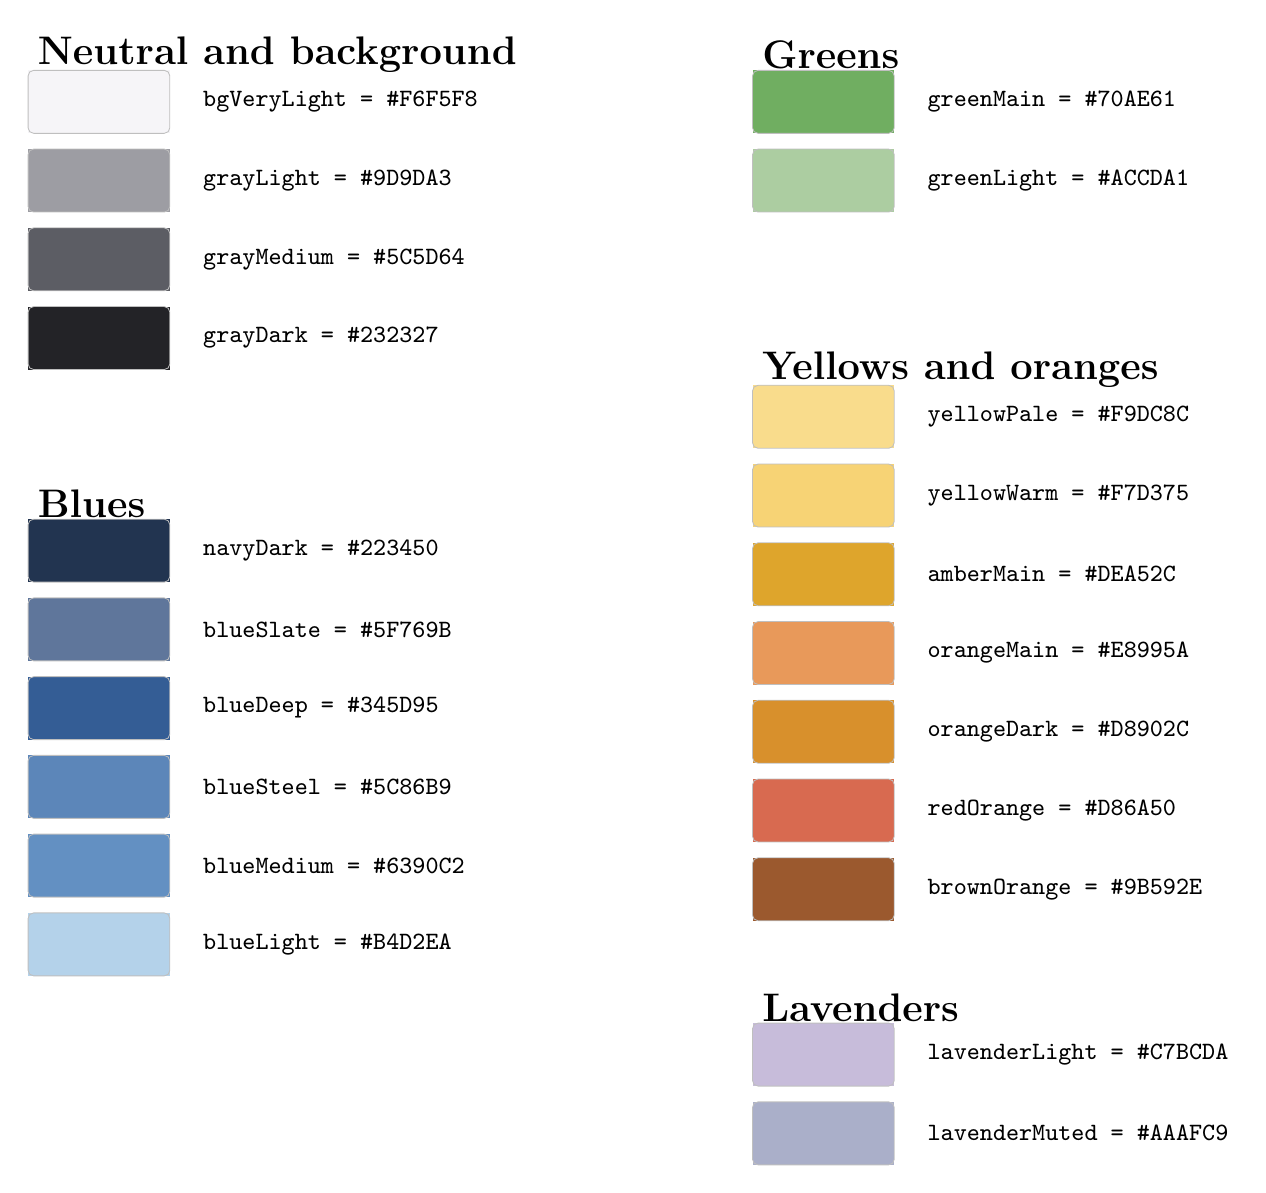
\begin{tikzpicture}[x=1cm,y=1cm]

		\tikzset{
            swatch/.style={
                rounded corners=2pt,
                draw=black!25,
                line width=0.3pt
            }
        }
        
        \newcommand{\ColorRow}[4]{
            \fill[#2] (#1,#3) rectangle ++(1.8,0.8);
            \draw[swatch] (#1,#3) rectangle ++(1.8,0.8);
            \node[anchor=west, font=\ttfamily\small] at (#1+2.1,#3+0.4) {#2 = #4};
        }
        
        \node[anchor=west, font=\bfseries\Large] at (0,12.8) {Neutral and background};
        
        \ColorRow{0}{bgVeryLight}{11.8}{\#F6F5F8}
        \ColorRow{0}{grayLight}{10.8}{\#9D9DA3}
        \ColorRow{0}{grayMedium}{9.8}{\#5C5D64}
        \ColorRow{0}{grayDark}{8.8}{\#232327}
        
        \node[anchor=west, font=\bfseries\Large] at (0,7.1) {Blues};
        
        \ColorRow{0}{navyDark}{6.1}{\#223450}
        \ColorRow{0}{blueSlate}{5.1}{\#5F769B}
        \ColorRow{0}{blueDeep}{4.1}{\#345D95}
        \ColorRow{0}{blueSteel}{3.1}{\#5C86B9}
        \ColorRow{0}{blueMedium}{2.1}{\#6390C2}
        \ColorRow{0}{blueLight}{1.1}{\#B4D2EA}
        
        \node[anchor=west, font=\bfseries\Large] at (9.2,12.8) {Greens};
        
        \ColorRow{9.2}{greenMain}{11.8}{\#70AE61}
        \ColorRow{9.2}{greenLight}{10.8}{\#ACCDA1}
        
        \node[anchor=west, font=\bfseries\Large] at (9.2,8.8) {Yellows and oranges};
        
        \ColorRow{9.2}{yellowPale}{7.8}{\#F9DC8C}
        \ColorRow{9.2}{yellowWarm}{6.8}{\#F7D375}
        \ColorRow{9.2}{amberMain}{5.8}{\#DEA52C}
        \ColorRow{9.2}{orangeMain}{4.8}{\#E8995A}
        \ColorRow{9.2}{orangeDark}{3.8}{\#D8902C}
        \ColorRow{9.2}{redOrange}{2.8}{\#D86A50}
        \ColorRow{9.2}{brownOrange}{1.8}{\#9B592E}
        
        \node[anchor=west, font=\bfseries\Large] at (9.2,0.7) {Lavenders};
        
        \ColorRow{9.2}{lavenderLight}{-0.3}{\#C7BCDA}
        \ColorRow{9.2}{lavenderMuted}{-1.3}{\#AAAFC9}
        
        \end{tikzpicture}
    \end{center}
    
    \vspace{0.5cm}
    
    \begin{center}
        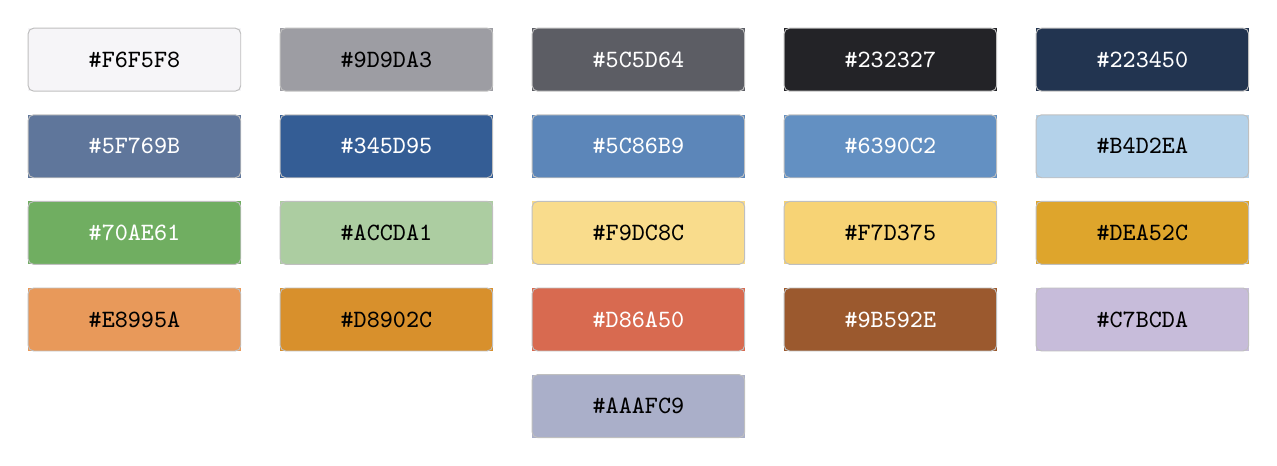
\begin{tikzpicture}[x=1cm,y=1cm]

            \tikzset{
                hexbox/.style={
                    rounded corners=2pt,
                    draw=black!25,
                    line width=0.35pt
                }
            }
            
            \newcommand{\HexBox}[5]{%
                \fill[#2] (#1,#3) rectangle ++(2.7,0.8);
                \draw[hexbox] (#1,#3) rectangle ++(2.7,0.8);
                \node[font=\ttfamily\small, text=#4] at (#1+1.35,#3+0.4) {#5};
            }
            
            \HexBox{0.0}{bgVeryLight}{5.0}{black}{\#F6F5F8}
            \HexBox{3.2}{grayLight}{5.0}{black}{\#9D9DA3}
            \HexBox{6.4}{grayMedium}{5.0}{white}{\#5C5D64}
            \HexBox{9.6}{grayDark}{5.0}{white}{\#232327}
            \HexBox{12.8}{navyDark}{5.0}{white}{\#223450}
            
            \HexBox{0.0}{blueSlate}{3.9}{white}{\#5F769B}
            \HexBox{3.2}{blueDeep}{3.9}{white}{\#345D95}
            \HexBox{6.4}{blueSteel}{3.9}{white}{\#5C86B9}
            \HexBox{9.6}{blueMedium}{3.9}{white}{\#6390C2}
            \HexBox{12.8}{blueLight}{3.9}{black}{\#B4D2EA}
            
            \HexBox{0.0}{greenMain}{2.8}{white}{\#70AE61}
            \HexBox{3.2}{greenLight}{2.8}{black}{\#ACCDA1}
            \HexBox{6.4}{yellowPale}{2.8}{black}{\#F9DC8C}
            \HexBox{9.6}{yellowWarm}{2.8}{black}{\#F7D375}
            \HexBox{12.8}{amberMain}{2.8}{black}{\#DEA52C}
            
            \HexBox{0.0}{orangeMain}{1.7}{black}{\#E8995A}
            \HexBox{3.2}{orangeDark}{1.7}{black}{\#D8902C}
            \HexBox{6.4}{redOrange}{1.7}{white}{\#D86A50}
            \HexBox{9.6}{brownOrange}{1.7}{white}{\#9B592E}
            \HexBox{12.8}{lavenderLight}{1.7}{black}{\#C7BCDA}
            
            \HexBox{6.4}{lavenderMuted}{0.6}{black}{\#AAAFC9}
        
        \end{tikzpicture}
    \end{center}
\end{document}